\item En este objetivo es en el que decidiremos nuestra hipótesis, la cual si recordamos era que no existía ninguna correlación entres los valores de nuestros registros.\\
Una vez que teniamos nuetra tabla filtrada por los datos pedidos en el objetivo anterior pasamos a obtener su coeficientes de correlación de Spearman, los cuales se muestran en la siguiente imagen \\
            \begin{figure}[h]
                \centering
                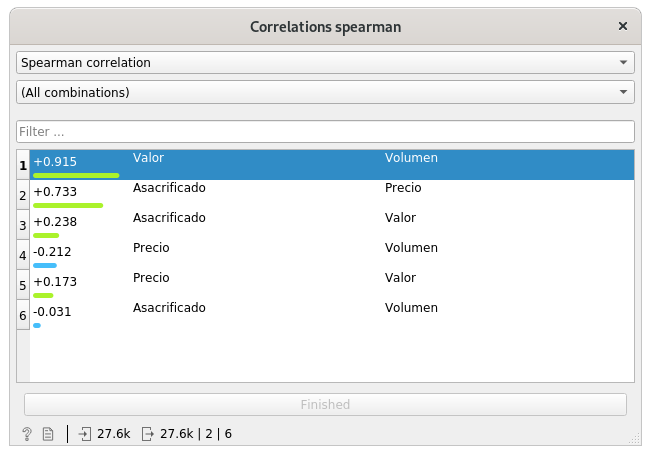
\includegraphics[scale = 0.3]{imagenes/correlacion.png}
                \caption{Correlación de Spearman}
                \label{correlacion}
            \end{figure}
\\Como podemos ver existen varias correlaciones, pero las más importantes son las existentes entre Valor-Volumen y Asacrificado-Precio, por lo cual podemos rechazar nuestra hipótesis.